%\documentclass[aspectratio=169]{beamer}
\documentclass[aspectratio=43]{beamer}
\usepackage{ucs}
\usepackage[T1]{fontenc}
\usepackage[utf8]{inputenc}
\usepackage[magyar]{babel}
\usepackage{amsfonts}
\usepackage{amsmath,bm}
\usepackage{amssymb}
\usepackage{graphicx}
%\usepackage{blindtext}
%\usepackage[hang]{caption}
%\usepackage{subcaption}
%\usepackage{blkarray,booktabs,bigstrut} % a címkézett mátrixhoz
%\usepackage{enumerate}
%\usepackage{psfrag}
%\usepackage[left=25mm,right=25mm,top=25mm,bottom=25mm]{geometry}
%\usepackage[hyphenbreaks]{breakurl}
%\usepackage[hyphens]{url}
%\usepackage{multirow}
%\usepackage{booktabs}
%\usepackage{hyperref}
%\usepackage{listings}
%\usepackage{cite}
%\usepackage{csquotes}
\usepackage{circuitikz}
\usepackage{siunitx}
\usepackage{xcolor}
%\usepackage[a-3u]{pdfx}

\definecolor{passgreen}{HTML}{00AA00}
\definecolor{stopred}{HTML}{AA0000}
%\definecolor{rosewood}{rgb}{0.6, 0.0, 0.04}
%\definecolor{indigo(dye)}{rgb}{0.0, 0.25, 0.42}

\usetheme{default}	% téma
\usefonttheme{serif}	% gyönyörű talpas betűtípus

\beamertemplatenavigationsymbolsempty % a pdf-be ágyazott navigációs gombok kikapcsolása
\newcommand\mat[1]{\underline{\underline{#1}}}

\title[Aktív tanulás, RF szűrő]{Koncentrált paraméterű\\ RF szűrő optimalizációja\\aktív tanulással} % cím
\subtitle[]{} 	% alcím
\date{\today}
\author[P.B., Sz.G.]{Pintér Bálint, Szilágyi Gábor}	% szerző
\institute{BME VIK} % intézmény vagy más infó a szerzőről

\begin{document}
\maketitle	% címoldal
\begin{frame}
	\frametitle{Az optimalizálandó hálózat egysége}
	%\framesubtitle{Az 1. dia alcíme}
    \begin{center}
    	\begin{circuitikz}[] %[longL/.style = {cute inductor, inductors/scale=0.75, inductors/width=1.6, inductors/coils=9}]
            \draw (-0.5,0)
            to[short, o-*] (2,0)
            to[short, -*] (2,0.5)
            to[short, -] (1,0.5);
            \draw (1,2.5)
            to[C, l=$C_{i,p}$] (1,0.5);
            \draw (2,2.5)
            to[short, -] (3,2.5)
            to[L, l=$L_{i,p}$] (3,0.5)
            to[short, -] (2,0.5);
            \draw (-0.5,3)
            to[short, o-*] (2,3)
            to[short, -*] (2,2.5)
            to[short, -] (1,2.5);
            \draw (2,0)
            to[short, -o] (8,0);
            \draw (2,3)
            to[short, -*] (5,3)
            to[short, -] (5,2)
            to[L, a=$L_{i,s}$] (7,2)
            to[short, -] (7,3);
            \draw (5,3)
            to[short, -] (5,4)
            to[C, a=$C_{i,s}$] (7,4)
            to[short, -*] (7,3)
            to[short, -o] (8,3);
            \draw[thick,red] (0,-0.5) rectangle (7.5,5);
        \end{circuitikz}
    \end{center}
\end{frame}
\begin{frame}
	\frametitle{Az egységhálózat helyettesítőképe}
	%\framesubtitle{Az 1. dia alcíme}
    \begin{center}
    	\begin{circuitikz}[] %[longL/.style = {cute inductor, inductors/scale=0.75, inductors/width=1.6, inductors/coils=9}]
            \draw (-0.5,0)
            to[short, o-*] (2,0)
            to[short, -] (2,0.5);
            \draw (2,2.5)
            to[generic, l=$Z_{i,p}(f)$] (2,0.5);
            \draw (-0.5,3)
            to[short, o-*] (2,3)
            to[short, -] (2,2.5);
            \draw (2,0)
            to[short, -o] (8,0);
            \draw (2,3)
            to[short, -] (5,3)
            to[generic, a=$Z_{i,s}(f)$] (7,3)
            to[short, -o] (8,3);
            \draw[thick,red] (0,-0.5) rectangle (7.5,3.5);
        \end{circuitikz}
    \end{center}
\end{frame}
\begin{frame}
	\frametitle{Az egységhálózat ABCD paraméterei ([a]-mátrixa)}
	%\framesubtitle{Az 1. dia alcíme}
    \begin{center}
    	\begin{circuitikz}[] %[longL/.style = {cute inductor, inductors/scale=0.75, inductors/width=1.6, inductors/coils=9}]
            \draw (-0.5,0)
            to[short, o-] (0,0);
            \draw (-0.5,3)
            to[short, o-] (0,3);
            \draw (7.5,0)
            to[short, -o] (8,0);
            \draw (7.5,3)
            to[short, -o] (8,3);
            \draw[thick,red] (0,-0.5) rectangle (7.5,3.5);
            \draw (3.75,1.5) node {$\mat{[a]_i}=\begin{bmatrix}a_{i,11}~a_{i,12} \\ a_{i,21}~a_{i,22}\end{bmatrix} \in \mathbb{C}^{2\times2}$};
        \end{circuitikz}
    \end{center}
\end{frame}
\begin{frame}
	\frametitle{Az optimalizálandó hálózat}
	%\framesubtitle{Az 1. dia alcíme}
    \begin{center}
    	\begin{circuitikz}[] %[longL/.style = {cute inductor, inductors/scale=0.75, inductors/width=1.6, inductors/coils=9}]
            \foreach \x in {1,...,5}
            {
                \draw (\x+\x-0.5,0)
                to[short, o-] (\x+\x+0,0);
                \draw (\x+\x-0.5,1)
                to[short, o-] (\x+\x+0,1);
                \draw[thick,red] (\x+\x+0,-0.2) rectangle (\x+\x+1,1.2);
                \draw (\x+\x+1,0)
                to[short, -o] (\x+\x+1.5,0);
                \draw (\x+\x+1,1)
                to[short, -o] (\x+\x+1.5,1);
                \draw (\x+\x+0.5,0.5) node {$\underline{\underline{[a]_{\x}}}$};
            }
        \end{circuitikz}
    \end{center}
\end{frame}
\begin{frame}
	\frametitle{Az optimalizálandó hálózat}
	%\framesubtitle{Az 1. dia alcíme}
    \begin{center}
    	\begin{circuitikz}[] %[longL/.style = {cute inductor, inductors/scale=0.75, inductors/width=1.6, inductors/coils=9}]
            \foreach \x in {1,...,5}
            {
                \draw (\x+\x-0.5,0)
                to[short, o-] (\x+\x+0,0);
                \draw (\x+\x-0.5,1)
                to[short, o-] (\x+\x+0,1);
                \draw[thick,red] (\x+\x+0,-0.2) rectangle (\x+\x+1,1.2);
                \draw (\x+\x+1,0)
                to[short, -o] (\x+\x+1.5,0);
                \draw (\x+\x+1,1)
                to[short, -o] (\x+\x+1.5,1);
                \draw (\x+\x+0.5,0.5) node {$\mat{[a]_{\x}}$};
            }
            \draw[thick,green] (1.75,-0.5) rectangle (11.25,1.5);    
        \end{circuitikz}
    \end{center}
    \begin{equation*}
        \mat{[a]} = \prod_{i}^{} \mat{[a]_{i}} = \begin{bmatrix}a_{11}~a_{12} \\ a_{21}~a_{22}\end{bmatrix} = \begin{bmatrix}A~B \\ C~D\end{bmatrix}
    \end{equation*}
    \vspace{1cm}\\
    Az egész hálózat $|S_{21}(f)|$ paraméterére vonatkozik specifikáció.\\
    \begin{equation*}
        S_{21} = \dfrac{2}{A+B/Z_0+C\cdot Z_0+D}
    \end{equation*}
\end{frame}
\begin{frame}
	\frametitle{A teljesítendő specifikáció}
	%\framesubtitle{Az 1. dia alcíme}
	\begin{columns}
		\column{0.4\textwidth}
			\begin{itemize}
				\item \textcolor{stopred}{Záró sáv}
				\item \textcolor{passgreen}{Áteresztő sáv}
				\item Átmeneti sáv (fehér)
				\item \textcolor{orange}{Extra büntetett régió}
			\end{itemize}
		\column{0.58\textwidth}
			\begin{figure}
				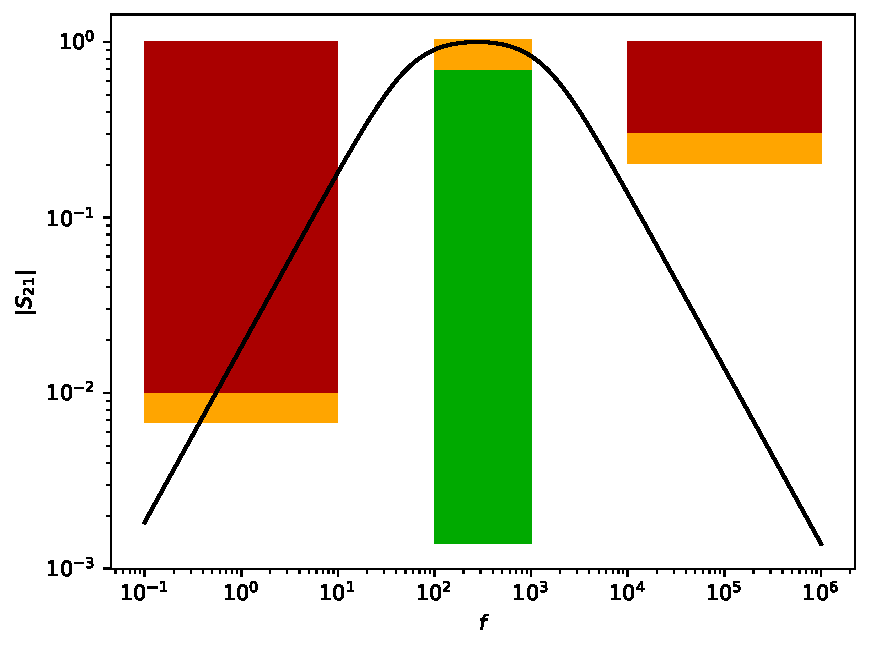
\includegraphics[width=\textwidth]{plot.pdf}
			\end{figure}
	\end{columns}
\end{frame}

\begin{frame}
	\frametitle{Bayesi optimalizálás}
	\begin{itemize}
		\item Specifikált probléma, költségfüggvény $\rightarrow$ optimális megoldás
		\item Nagy szabadsági fok, kiértékelés költséges, bonyolult, időigényes lehet
		\item Bayesi optimalizálás, megoldásához: már létező könyvtár\\
		(Bayesian Optimization lib, ami a scikit-learn-ön alapul)
	\end{itemize}
	\begin{figure}
		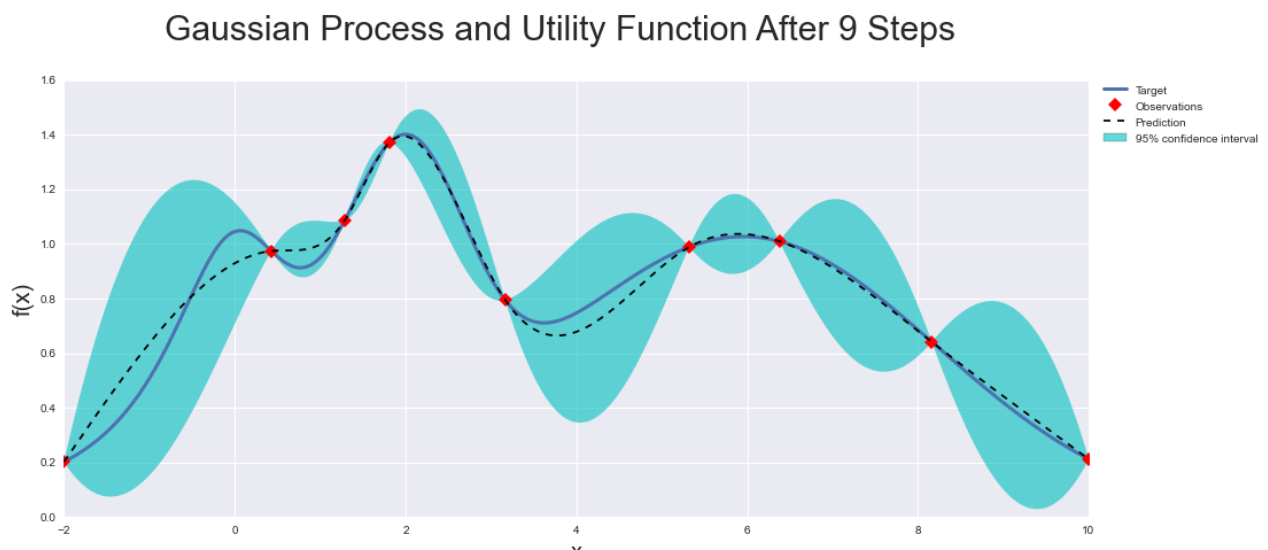
\includegraphics[width=0.9\textwidth]{gauss.PNG}
	\end{figure}
\end{frame}

\begin{frame}
	\frametitle{Bayesian Optimization könyvtár}
	\begin{itemize}
		\item Példányosítás, inputok: költségfüggvény, határok 
		(maximalizálás)
		\item \textit{maximize( )} függvény, inputok: kezdeti random pontok, iterációszám
		\item Ebben: \textit{utility} függvény definiálás, majd iteratív megoldás
	\end{itemize}
	\pause
	Minden iterációs lépésben:
	\begin{itemize}
		\item Paraméterfrissítés: \textit{update\_param()} tagfüggvény
		\item frissített \textit{utility}-val javaslat (\textit{suggest( )}) egy új kiértékelési helyre, \textit{x\_probe}-ra
		\item \textit{probe( )} kiértékeli \textit{x\_probe} helyen
	\end{itemize}
	Iteráció lefut: maximalizált pont a paramétertérben.
\end{frame}

\begin{frame}
	\frametitle{Paraméterfrissítés}
	\textit{Utility} függvény \textit{update\_param} tagfüggvénye:
	\begin{itemize}
		\item Feltárási stratégia: UCB, EI, POI\\alapbeállítás: UCB (Upper Confidence Bounds method)
		\item $\kappa, \chi$ hiperparaméterek
		\item $\kappa_{decay}$-vel szorozódik (csökken) $\kappa$ minden $\kappa_{decay-delay}$ utáni iterációban
	\end{itemize}
\end{frame}

\begin{frame}
	\frametitle{Új kiértékelési hely javaslat}
	\textit{Suggest( )} javaslata = \textit{argmax( )}-ot néz egy akvizíciós függvényre, \textit{acq\_max}-ra
	\begin{itemize}
		\item Input: \textit{utility} függvény
		\item Első lépés: mintavételezés $10^5$ pontra, random, egyenletes eloszlással
		\item Második lépés: L-BFGS-B optimalizációs metódus (minden mintavételezési pontra)
		\item Visszatér az legnagyobbal, ez lesz: \textit{x\_probe}
	\end{itemize}
\end{frame}

\begin{frame}
	\frametitle{L-BFGS-B optimalizáció}
	\begin{itemize}
		\item L-BFGS-B solver: \textit{scipy.optimizer} könyvtárból, minimalizálási feladatokra $\rightarrow$ módosítani kell \textit{acq\_max}-ot
		\item Másodrendű optimalizációs algoritmus, Kvázi-Newton módszer
		\item L-BFGS algoritmus (Limited-memory Broyden-Fletcher-Goldfarb-Shanno) kiterjesztése korlátok kezelésével
		\item Másodrendű deriváltat közelít, ahol azt közvetlenül nem lehet kiszámolni
		\item Nem kell kiszámolni a Hesse-mátrixot\\(csak $\underline{\underline{H}}^{-1}$-t közelíti)
		\item Limitált memória: csak az elmúlt \textit{m} lépés koordináta- és gradiensvektorát tárolja el.
	\end{itemize}
	
\end{frame}

%\begin{frame}
%	\frametitle{Az egydimenziós modell}
%	\begin{columns}
%		\column{0.48\textwidth}
%			A következő egyszerűsítésekkel jutunk 3D-ből az 1D plazmához: \\
%			\begin{itemize}
%				\item A töltetlen $Xe$ részecskéket elhagyjuk
%				\item Az ütközésektől eltekintünk
%				\item Csak az elektronok mozgását vizsgáljuk
%				\item Pontszerű részecskék helyett felületi töltéssűrűséggel rendelkező, az $x$ tengelyre merőleges lapok
%				\item A pozitív töltésű $Xe^+$ ionokat helyhez kötött háttér-töltéssűrűségnek vesszük
%			\end{itemize}
%		\column{0.48\textwidth}
%			\begin{itemize}
%				\item A szimulációs tér egydimenziós és ciklikus, $x=0 \Longleftrightarrow x=N_g$
%				\item A külső elektromos teret 0-nak vesszük
%				\item A mégneses térnek nincs hatása 1D-ben
%			\end{itemize}
%	\end{columns}
%\end{frame}
%\begin{frame}
%	\frametitle{A Particle-Mesh módszer}
%	\begin{columns}
%		\column{0.48\textwidth}
%			\begin{itemize}
%				\item item
%			\end{itemize}
%		\column{0.48\textwidth}
%			\begin{figure}
%				\includegraphics[width=\textwidth]{/home/g/Pictures/nap.png}
%			\end{figure}
%	\end{columns}
%\end{frame}
\end{document}
